\documentclass[11pt,letterpaper]{article}

\usepackage{graphicx}
\graphicspath{{images/}}
\usepackage{longtable}
\usepackage{float}
\usepackage{tabu}
\usepackage{fancyhdr}
\usepackage{geometry}

%margin
 \geometry{
 left=25mm,
 right=25mm,
 top=25mm,
 bottom=25mm,
 }

\pagestyle{fancy}
%\renewcommand{\headrulewidth}{0pt}
\lhead{Hadoop - Content based Search \& Retrieval}
\rhead{Software Requirement Specification}

%Title Page
\title{
	\textbf{Hadoop add-on API for Advance Content Based Search \& Retrieval} \\
	Software Requirement Specification
}

\date{
	2015-08-29
}

\author{
	\textbf{Developers}\\
	Kshama Jain \\
	Aditya Kamble \\
	Siddhesh Palande \\
	Rahul Rao
}

\begin{document}

\maketitle
\newpage

\tableofcontents
\newpage


\section{Introduction}


\subsection{Project Scope}

\paragraph{}
This system shall retrieve the required contents of files which are in an unstructured format containing huge amount of Data like e-books in a digital library where the number of books are present in thousands. The scope here is initially limited to PDF files which may be expanded to other unstructured formats like ePUB, mobi.  

\paragraph{}
The input is provided to the system API in the form of search query which will be firstly filtered to find the important expression as a query to the API which will return the important content to the user in the form of paragraph or text highlighted using the power of distributed computing. 

\paragraph{}
The particular page or the Entire book itself can be downloaded by the Library users if the content is satisfied else the search continues for finding relevant content 

\subsection{User Classes and Characteristics}

\paragraph{}
The end user of this system will be Application Developer who will be using the API provided along with the Hadoop as an Add-on (Plugin) along with the set of Hadoop API which will be indirectly be accessed by the people accessing the digital library system application created by the application developer.

\begin{itemize}
\item Developer
\item Librarian
\item Library Users
\end{itemize}

\subsection{Operating Environment}

\paragraph{}
The environment here is assumed to be distributed with a cluster having n number of Computers connected together to form a Hadoop Cluster with Hadoop HDFS as well as HBASE NOSQL Database installed for storing metadata of each PDF being pushed and HDFS formatted File system containing huge amount of digital eBooks.

\paragraph{}
The job of server application here is just to push the eBooks (PDF Files) in the Hadoop File System which will be distributed among the nodes forming the Hadoop cluster.

\subsection{Design and Implementation Constraints}

\begin{itemize}
\item Along with Hadoop Implementation an add-on in the form of JAR library shall be included by the developer using this system which will provide API for high speed retrieval of relevant content. This API will basically assume to be a multinode cluster installed in the deployed environment.
\item The data store API for content based retrieval shall be purely implemented in JAVA which on future shall be implemented for Python and C++ as well.
\item There will be basic tokenization of input string and numerous possibilities will be searched distributively on various nodes using the map reduce.
\item The final result shall be obtained by the master node and will be passed on to the client application for viewing the results.
\item On a future note, Apache spark shall be used to implement this system for speed incremental purposes in case of limitations in the speed of map reduce algorithm.
\end{itemize}

\subsection{Assumptions and Dependencies}

\begin{enumerate}
\item UBUNTU 14.04.2 LTS workstation edition on the master node or namenode having a monitor for viewing the Interface by the application user.
\item UBUNTU 14.04.2 LTS Server edition or minimalistic UBUNTU 14.04.2 on datanodes and secondary namenode.
\item JDK 1.7 and above
\item Hadoop 2.6.x and above
\item Browser Any
\item OPENSSH-server on all nodes
\item Virtualization enabled for pseudo distributed (testing purposes only).
\item VMWARE/Virtual box/oVirt Virtualization managers installed.
\end{enumerate}


\newpage

\section{System Features}

{\tabulinesep=2mm
   \begin{longtabu} { |p{5cm} | p{5cm} | p{5cm }|}
       \hline

\textbf{Requirement ID} & \textbf{ Requirement} & \textbf{Requirement Description}\\ \hline
	
FR01 &
Entering the keyword/s &
User will have to enter keyword/s in the search box in order to obtain desired results, system should take 	 the keyword input and validate it and search the metadata.\\ \hline

FR02 & Add a document to the system & User simply needs to upload a file on the system. The system should create an appropriate metadata from it and store it in the index.\\ \hline

FR03 & Ranking the documents & System should use a ranking algorithm to rank the documents stored in it. It may contain more page hits and other factors required for ranking.\\ \hline

FR04 & Retrieving  the content from the database & On finding the most relevant documents corresponding to the user’s query, system should give the content to the user in the form of pages from top ranking documents. Top ranking documents would be the ones which have more number of matching keywords.\\ \hline

FR05 & 
Indexing the Data/Creating a metadata & 
Whenever the user uploads a file or updates, system should read the file create a metadata for a new file by adding the ‘title’ as an index and for an update it should check the changes and update the title of the same.\\ \hline

FR06 &
Validating a keyword & 
User may make a mistake like some use of unnecessary words or some spelling mistake while entering a keyword, system should validate that keyword and fine the most relevant keyword from the given input. For this operation system should use a validating keyword algorithm.\\ \hline

FR07 & 
Downloading the content & 
When a user finds the necessary content, system should ask him how he/she wants the content to be retrieved, whether the complete document or that same page or some more pages before and after that page.\\ \hline
      
   \end{longtabu}
}


\newpage


\section{External Interface Requirements}

\subsection{User Interfaces}

\begin{itemize}
\item The User Interfaces are to designed and written by the developer who will be using the API. The sample application provided along with the Hadoop API built on either GTK, Java Swing or Java FX.
\item This system shall have an input text box which will be used for taking the input from the user.
\item There shall be a progress bar of the search going on in the bottom of interface indicating the number of documents processed in terms of percentage.
\item Also there shall be a provision for Highlighting the particular keywords user gave as input and to view the surrounding contents by scrolling the document.
\item A next button will increment the search result obtained by 10. 
\item On clicking on a results list item , the user can view the particular result along with book 
\item Title and page number and total number of pages and size of book.
\item On right clicking on a result, there shall be three options.

	\begin{enumerate}
	\item Download current page
	\item Download pages entered
	\item Download Entire book
	\end{enumerate}

\end{itemize}

\subsection{Hardware Interfaces}

\begin{itemize}
\item There shall be N number of nodes each having the following hardware configuration in a fully distributed system connected environment together in a wired manner using Ethernet interface.
\item Intel i3/i5/i7 processor
\item Ethernet Interface on NIC
\item Virtualization of upto 2 or 3 nodes on a single machine for testing purposes
\item 2 or 4 GB RAM (and upto 512 MB for each node for pseudo disrtibuted)
\end{itemize}

\subsection{Software Interfaces}

\begin{itemize}
\item Any Open Source Linux Distribution.(Ubuntu Server version 14.04.2 Preferred)
\item OPENSSH installed on each machine with public key of each node in authorized\_keys directory along with the localhost.
\item JDK Version 1.7 or above
\item JAVA\_HOME to be appended in the \$PATH environment variable
\item Hostname to be initialized for each node in the /etc/hosts file having a masternode (namenode), secondary namenode and various slave nodes to be added.
\item \$HADOOP\_HOME environment variable path to added in the ~/.bashrc 
\item Following Files to be configured in \$HADOOP\_HOME/etc/hadoop directory

	\begin{enumerate}
	\item core-site.xml
	\item hadoop-env.sh
	\item yarn-site.xml
	\item mapred-site.xml
	\item master
	\item slave
	\end{enumerate}

\item Master node with Ubuntu Workstation version preferred for supporting Eclipse IDE with Hadoop plugin for development and Server having Ubuntu Server version Preferred.
\end{itemize}

\subsection{Communication Interfaces}

\begin{itemize}
\item All the nodes are connected through Ethernet cables using eth0 interface.
\end{itemize}

\newpage

\section{Nonfunctional Requirements}

\subsection{Performance Requirements}
	
Memory Requirements:
\begin{itemize}	
\item Memory require for Hadoop installation and HBase and Map Reduce components.
\item API requires minimum 100 MB space as it contains core components for content based retrieval
\item 4 GB Primary Memory / RAM
\end{itemize}

Speed Requirements:
\begin{itemize}
\item Intel i3/i5/i7 64bit or AMD Processors
\end{itemize}

\subsection{Security Requirements}
\begin{itemize}
\item SSH Authentication to communicate with Namenode and Datanodes
\end{itemize}

\subsection{Software Quality Attributes}

\paragraph{}
Software Quality can be defined as “the conformance to explicitly stated functional and performance requirements, explicitly documented development standards, and implicit characteristics that are expected of all professionally developed software”.\\
	
\textbf{Software Quality Attributes are}

\begin{enumerate}
\item \textbf{Functionality}
\paragraph{}
This is an ability by which the software satisfies the needs of the software denoted by suitability, accuracy, interoperability, compliance and security.

\item \textbf{Reliability}
\paragraph{}
Due to wired connectivity, reliability can be guaranteed.

\item \textbf{Availability}
\paragraph{}
The system should be available during their respected hours.

\item \textbf{Usability}
\paragraph{}
This ability indicates that the usefulness of the software.

\item \textbf{Efficiency}
\paragraph{}    
This indicates the measure of computing resources and time required by the program to perform.

\item \textbf{Maintainability}
\paragraph{}
The ability required to locate or fix bugs in software. There should be facility to add or delete or update documents.

\item \textbf{Portability}
\paragraph{}
The software works properly even if the environment gets changed (i.e. change in hardware or software).

\item \textbf{Reusability}
\paragraph{}
With new versions of Hadoop this API can be improved using new features of Hadoop

\end{enumerate}

\newpage

\section{Other Requirements}

\subsection{Database Requirements}
\paragraph{}
\textbf{HBase} – HBase is distributed database and compatible with \textbf{Hadoop} distributed system. It is required to implement indexing the content present in \textbf{HDFS}. It is basic requirement that HBase should be present on the system to use this software. Our API contains methods to retrieve data from content and it will speed up using indexing. 

\subsection{Internalization Requirements}
\begin{figure}[h]
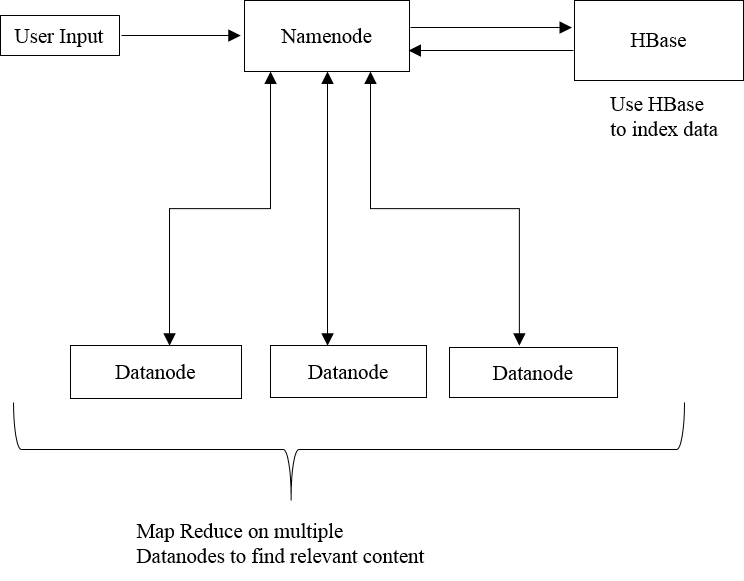
\includegraphics{internalization}
\centering
\end{figure}

\subsection{Legal Requirements}
\textbf{Hadoop} is an open source project and this API based on Hadoop will also be open source. It will be released under Apache License. Customer should be aware of Apache License before using this application.

\subsection{Reuse Objectives for the Project}
\begin{itemize}
\item This API can be extended to perform content based retrieval of  ePub and mobi files
\item With new versions of Hadoop this API can be improved using new features of Hadoop
\end{itemize}

\newpage

\section{Analysis Model}

\subsection{Data Flow Diagrams}
\begin{figure}[H]
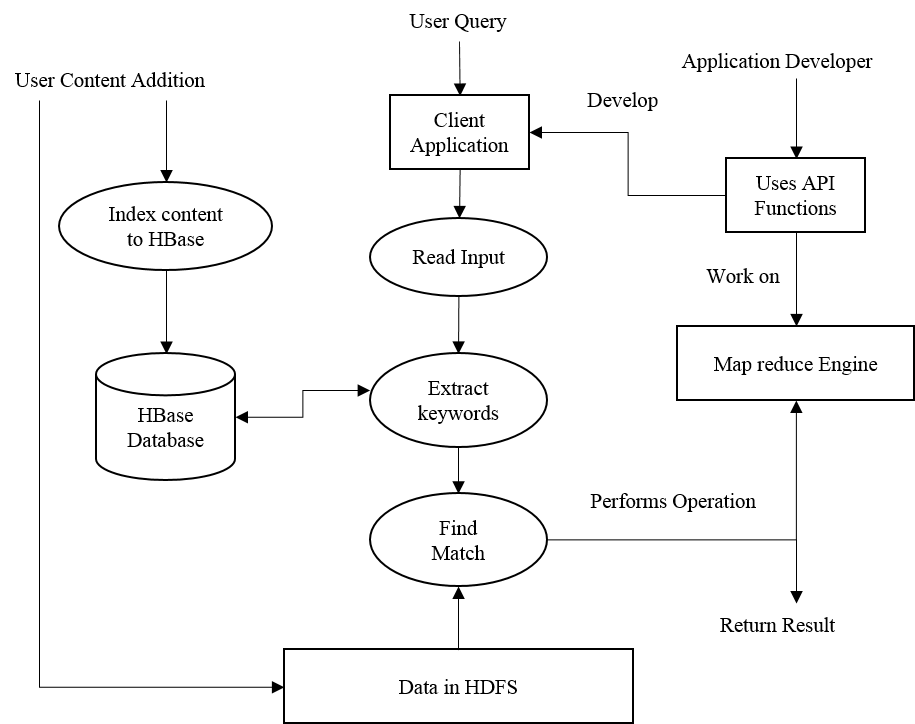
\includegraphics{data_flow}
\centering
\end{figure}

\newpage

\subsection{Class Diagrams}
\begin{figure}[H]
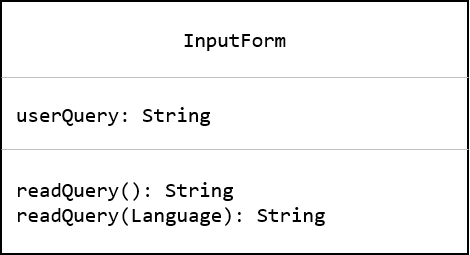
\includegraphics{class_input_form}
\centering
\end{figure}

\begin{figure}[H]
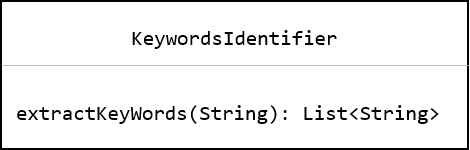
\includegraphics{class_keyword_identifier}
\centering
\end{figure}

\begin{figure}[H]
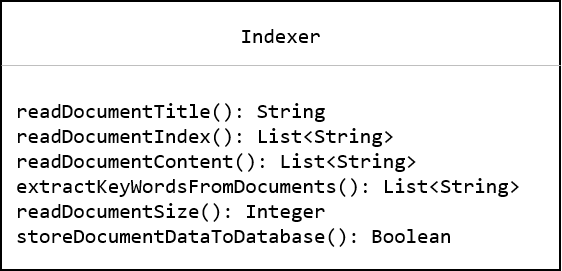
\includegraphics{class_indexer}
\centering
\end{figure}

\begin{figure}[H]
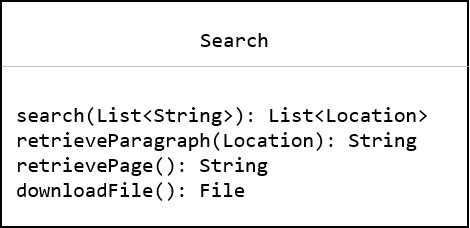
\includegraphics{class_search}
\centering
\end{figure}

\begin{figure}[H]
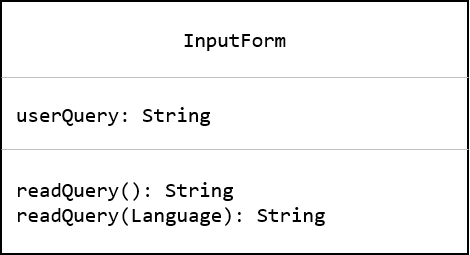
\includegraphics{class_input_form}
\centering
\end{figure}

\begin{figure}[H]
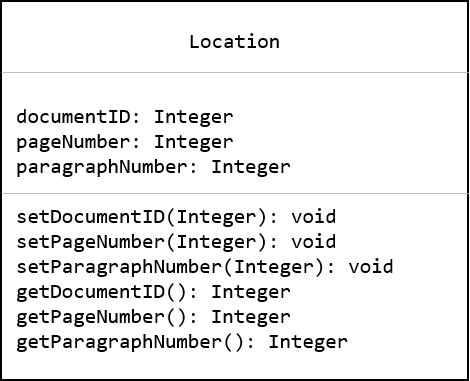
\includegraphics{class_location}
\centering
\end{figure}

\newpage

\subsection{Entity Relationship Diagrams}
\begin{figure}[H]
	\makebox[\textwidth]{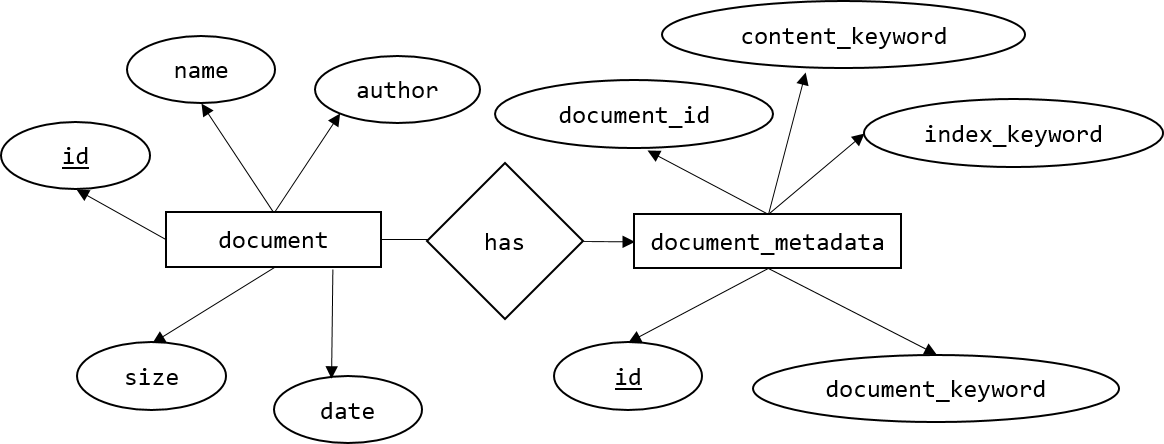
\includegraphics{entity_relationship}}
\centering
\end{figure}

\newpage

\section{System Implementation Plan}

 {\tabulinesep=2mm
   \begin{tabu} {|c|c|c|c|}
       \hline

	\textbf{Activity} & \textbf{Weeks to Spend} & \textbf{Deliverables} & \textbf{Priority}\\ \hline
	Analysis of Existing System & 2 weeks & - & Normal \\ \hline
	Requirement Gathering & 2 weeks & Requirements & Normal \\ \hline 
	Literature Survey & 3 Week & - & Normal \\ \hline
	Designing and Planning & 5 weeks & Modules & High \\ \hline
	Implementation & 16 weeks & API & High \\ \hline
	Testing & 3 weeks & Test Report & High \\ \hline
	Documentation & 4 week & Project Report & Normal \\ \hline
      
   \end{tabu}
}

\end{document}
